\documentclass{article}

%packages
\usepackage{graphicx}
\usepackage{tikz}
\usepackage[utf8]{inputenc}
\usepackage{amssymb}

\begin{document}

\usetikzlibrary{automata,arrows, positioning}
\renewcommand{\contentsname}{Tabla de contenidos}

\begin{titlepage}
	\begin{center}
		
\includegraphics{./images/escudo.jpg}
	\end{center}
	\centering
	{\scshape\LARGE Complutense de Madrid \par}
	\vspace{1cm}
	{\scshape\Large Práctica Programación Evolutiva.\par}
	\vspace{1.5cm}
	{\huge\bfseries Primera práctica. \par}
	\vspace{2cm}
	{\Large\itshape Raúl Torrijos \& Lukas Häring\par}
	%{\large Grupo 9\par}
	\vfill
	\vfill

% Bottom of the page
	{\large \today\par}
\end{titlepage}

\tableofcontents


\section{Introducción}
En esta práctica vamos a realizar una búsqueda de mínimo/máximos utilizando una técnica evolutiva basada en chromosomas . Los chromosomas pueden ser \textit{binarios}, basados en vectores de 0s y 1s para los genes, o \textit{reales}, basados en elementos Doble (Valores de coma flotante). Constan de 4 etapas (\textit{GeneticAlgorithm.java}), \textbf{evaluación}, dónde los chromosomas se evalúan, utilizando las técnicas vistas en los pdf; \textbf{selección}, dónde se elige utilizando un criterio a los descendientes, en nuestra práctica, \textit{Ruleta}, \textit{Torneo Determinista} y \textit{Torneo Probabilista}; \textbf{Cruce}, de los candidatos elegidos, algunos se "mezclarán" (dos a dos) y crearán dos chromosomas distintos (dando mayor variabilidad); \textbf{Mutación}, muta aleatoriamente, en el caso de ser un chromosoma \textit{Binario}, bits del vector, si este es \textit{Real} existen dos tipos de mutación, una mutación de mínimo desplazamiento, se elige la bola más próxima al extremo y se genera un número aleatorio, o una mutación aleatoria, dónde un gen es reemplazado por otro valor distinto al que había.

En la práctica podemos seleccionar el elitismo, es decir, asegurarnos de que un subconjunto de cromosomas con mejor evaluación siempre son tambíen descendientes puros (Sin modificarse).

\newpage

\section{Ejemplos}
Todos estos ejemplos se han realizado con los siguientes valores: un \textbf{Tamaño de población} de \textbf{100}; un \textbf{Número de generaciones} de \textbf{100}; un \textbf{60\%} de \textbf{Cruces}; un \textbf{5\%} de \textbf{Mutaciones} y una precisión para los chromosomas binarios de \textbf{0.0001}.
\subsection{Función 1}
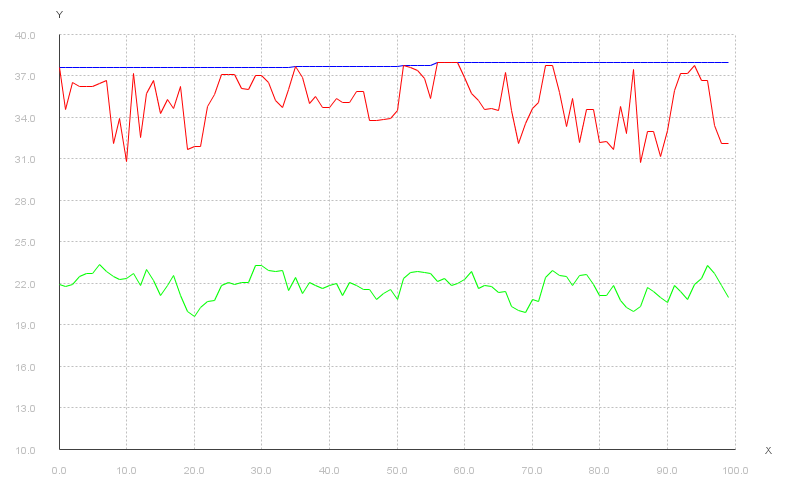
\includegraphics[scale=0.5]{./images/graph1_bin.png}
Los valores de

\subsection{Función 2}
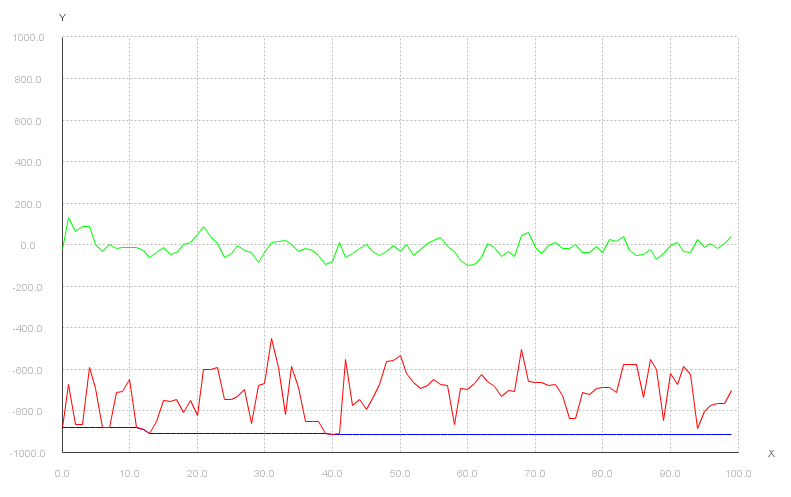
\includegraphics[scale=0.5]{./images/graph2_bin.png}

\subsection{Función 3}
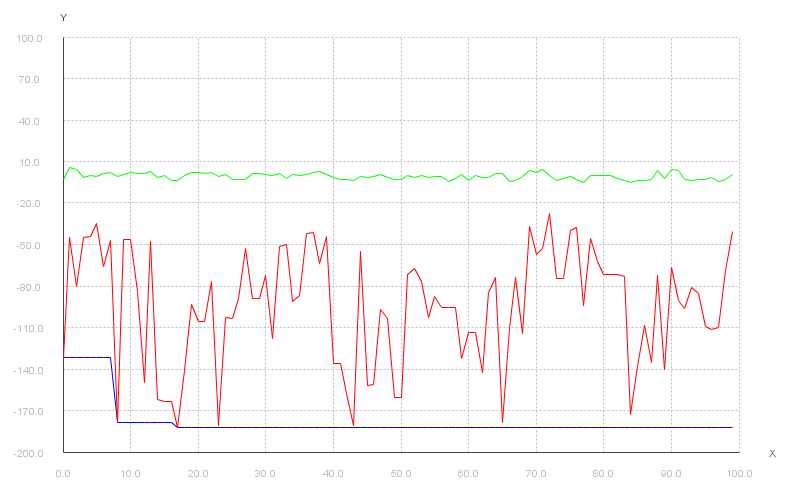
\includegraphics[scale=0.5]{./images/graph3_bin.png}

\subsection{Función 4}
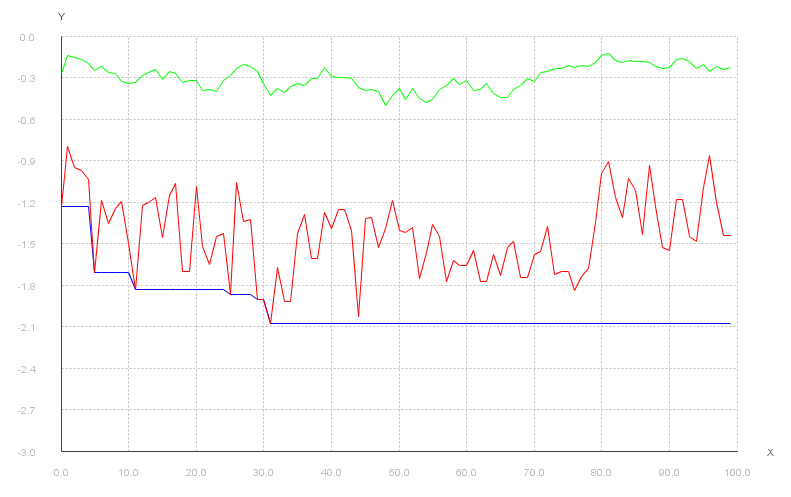
\includegraphics[scale=0.5]{./images/graph4_bin.png}
Como podemos ver, se puede cambiar el número de argumentos a través del panel de control.

\subsection{Elitismo}
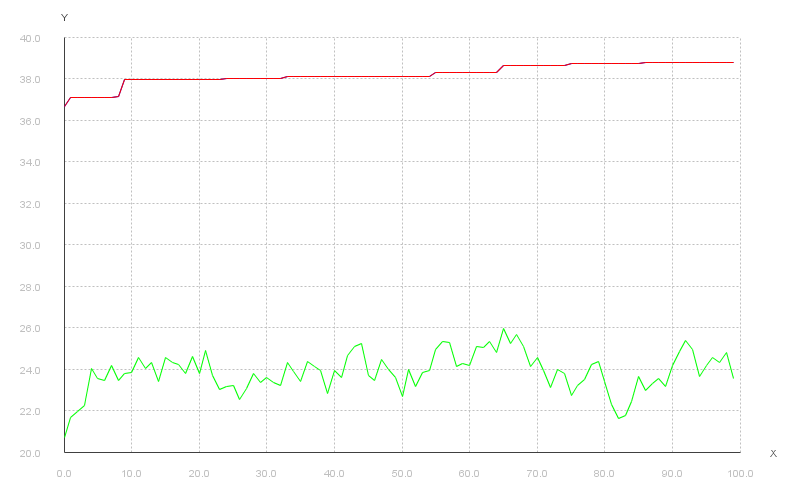
\includegraphics[scale=0.5]{./images/graph1_eli.png}
Como podemos ver, el mejor absoluto coincide con el mejor de la generación, esto es ya que siempre nos aseguramos que el mejor de la generación anterior siempre desciende o mejora, por lo que siempre va a estar ahí.

\end{document}
